% MCI_Report
\documentclass[]{aastex63}

\usepackage{amsmath}
\usepackage{graphicx}
\usepackage{hyperref}

\begin{document}
\title{Multi-Color Imaging of Messier 81 with the Vassar College Class of 1951 Observatory}

\author{Mariah C. Jones}
\affiliation{Vassar College \\
124 Raymond Avenue\\
Poughkeepsie, NY 12604, USA}

\begin{abstract}
This report details the multi-color imaging of Messier 81 (M 81), also known as Bode's Galaxy, conducted with the Vassar College Class of 1951 Observatory. Utilizing a 32-inch reflecting telescope equipped with research-grade electronic cameras and spectrographs, observations were made in blue, green, red, and yellow filters to produce a comprehensive multi-colored image. The data acquisition process, including calibration frames such as flats, darks, and biases, was meticulously documented and executed. Challenges encountered during data reduction, including inconsistencies in file organization and filter performance, were addressed, resulting in a final multi-color image. Analysis of the final image revealed insights into the brightness distribution and structure of M 81, highlighting the galaxy's spiral arms and central bulge. Additionally, calculations based on the apparent and absolute magnitudes of M 81 yielded valuable astrophysical parameters. This project not only enhanced observational skills but also provided valuable insights into the properties and behavior of spiral galaxies like M 81.
\end{abstract}

\section{Introduction}
The Vassar College Class of 1951 observatory has a 32-inch reflecting telescope, equipped with research-grade electronic cameras and three spectrographs, and is one of the largest research telescopes in New York State \citep{vassar}. Since its construction in 1997, the observatory has been used for public outreach and education, professional research, and student coursework alike \citep{vassar}. Most recently, my ASTR240 classmates and I were tasked with observing an object in four different filters to produce a multi-colored image, and we chose to observe Messier 81 (M 81), also known as Bode's Galaxy. We selected blue, green, red, and yellow-colored filters, which block out certain kinds of light. This allows us to see how bright an object is in a certain color, or to look at a specific spectral line of an element, like H $\alpha$ \citep{iowa}. First observed by German astronomer Johann Elert Bode in 1774 \citep{nasa}, M 81 is a spiral galaxy similar to the Milky Way \citep{brandt} in size, mass, and shape \citep{Brunthaler}. It also has a nuclear radio source, M 81*, speculated to be a supermassive black hole similar to Sgr A*, the supermassive black hole at the center of the Milky Way. Located in the constellation Ursa Major, the galaxy is relatively close to the Earth, being roughly 3.6 Mpc away \citep{Gurzadyan}. This Messier object has a right ascension of 9$h$:55:33 and declination of + 69$^{\circ}$ \citep{simbad}, resulting in spring being the best time to see it \citep{nasa}. On 25 March of this year, we were able to take images and calibration frames with different filters of M 81, allowing us to later reduce the data by applying calibration corrections to produce a multi-color image.

\section{Observations and Data Reduction}
Zoe and I completed an observing shift together, where I was in charge of updating the log and Zoe handled the imaging. While I received guidance from Elyse, Zoe, and Prof. Salyk, I completed the data reduction alone. 

\subsection{Observing}
% flats
In order to begin collecting data, we first had to calibrate the telescope and ensure our object was centered. Once the instrument was properly set up, we were able to begin acquiring and recording data. The log, used to document the acquisition process, included the following columns to help keep things organized for future data reducing ; file name, object, filter, exposure, universal time (UT) start, and comments. Our first runs were just flat frames of each filter color, which would later be used to improve the data. A flat frame is an image taken that has uniform lighting across the entire frame, and it ensures that each pixel will give the same value when exposed to the same amount of light. We take a number of flats with different exposures to stack and create a master flat field to divide our data by, which will allow us to mathematically remove obstructions that might be on a sensor or filter, like dust or smudges, ultimately reducing noise. Flats can be taken by pointing the telescope at a source able to evenly illuminate the field of view, and should be captured in the same conditions that raw images were taken in.
\\
\\
% darks
After making flats for each filter, we then made dark frames which will eventually be subtracted from the data. Similar to flats, dark frames ensure all pixels give the same value when not exposed to light by capturing the random noise created by the sensor itself. A longer exposure time correlates to a higher amount of random photons produced from the sensor, so by only capturing this random noise, we improve our data and reduce noise by subtracting the dark frames. We took darks with exposures matching our flats and stack them to create a master dark, which is what gets subtracted. Darks can be created by taking images, while the telescope is covered, in the same conditions that raw images are taken in. 
\\
\\
% raw images
With flats and darks created, we were able to begin imaging our object, M 81. Certain filters were missing and others were damaged, so we decided to use the red, green, yellow, and blue; the blue filter produced abnormal striations on the images. After putting the desired filter into place, we took a test image to determine the exposure time needed for each filter. To determine an exposure time, we set the test image's exposure to 10 seconds and checked the maximum illumination of the sensor, or the maximum number of photons collected. To ensure our images were not over-saturated, we chose an exposure time that would allow the sensor to collect just under the maximum amount of photons possible; the r filter has an exposure of 40 seconds, green and yellow have 60 seconds, and blue has 75 seconds. A minimum of three images was taken of each filter, saved and uploaded to a shared Google drive, and recorded in the log.

\subsection{Reduction}
% bias
The last kind of calibration frame used to improve data is known as the bias frame, which calibrates the sensor's readout noise. Bias frames are very similar to dark frames, the difference being that bias frames have no exposure time. I was able to account for and subtract bias when reducing the data using two \href{https://github.com/mariahjones/ASTR240_MCI}{Jupyter Notebooks}. In the notebooks, I first subtract the bias frames from the raw and dark images to eliminate bias, then I create a master dark by combining each dark into one. I then process each of the flats by reducing, combining, and producing a compiled master flat for each filter. With the master dark subtracted from each flat, I am able to inspect each master flat to ensure the process worked.
\\
\\
% reduction
Once I confirm everything functions as desired, I begin reducing the data files, which entails subtracting the master dark from the raw images, and then divide the difference by the master flat correlating to each filter to maintain CCD consistency. I then created a plot of the reduced image that I compared to my raw image to ensure the reduction worked properly. The reduced image has subtle differences from the raw image, one of them being the elimination of visible dust donuts due to the flat frame calibration.

\begin{figure}[h]
    \centering
    \includegraphics[scale=.6]{raw_vs_reduced_v.png}
    \caption{A plot comparing a raw image, taken with the green filter, to the reduced image. The reduction process includes subtracting the master bias and master dark frames from the data files, and then dividing the data by the master green flat frame. Note the subtle differences between the two images; the raw image includes dust and striations that the reduced image does not, ultimately resulting in a more clear scan.}
    \label{fig:comparison}
\end{figure}

With the reduction process working as expected, I am able to reduce each raw image with a function looping through each file, and I then shift and align the files for each filter, plotting the shifted images to make sure everything looks right, in preparation for the final step. Lastly, with the images from each filter completed, I stack the images in order to produce the single multi-color image.

\begin{figure}[h]
    \centering
    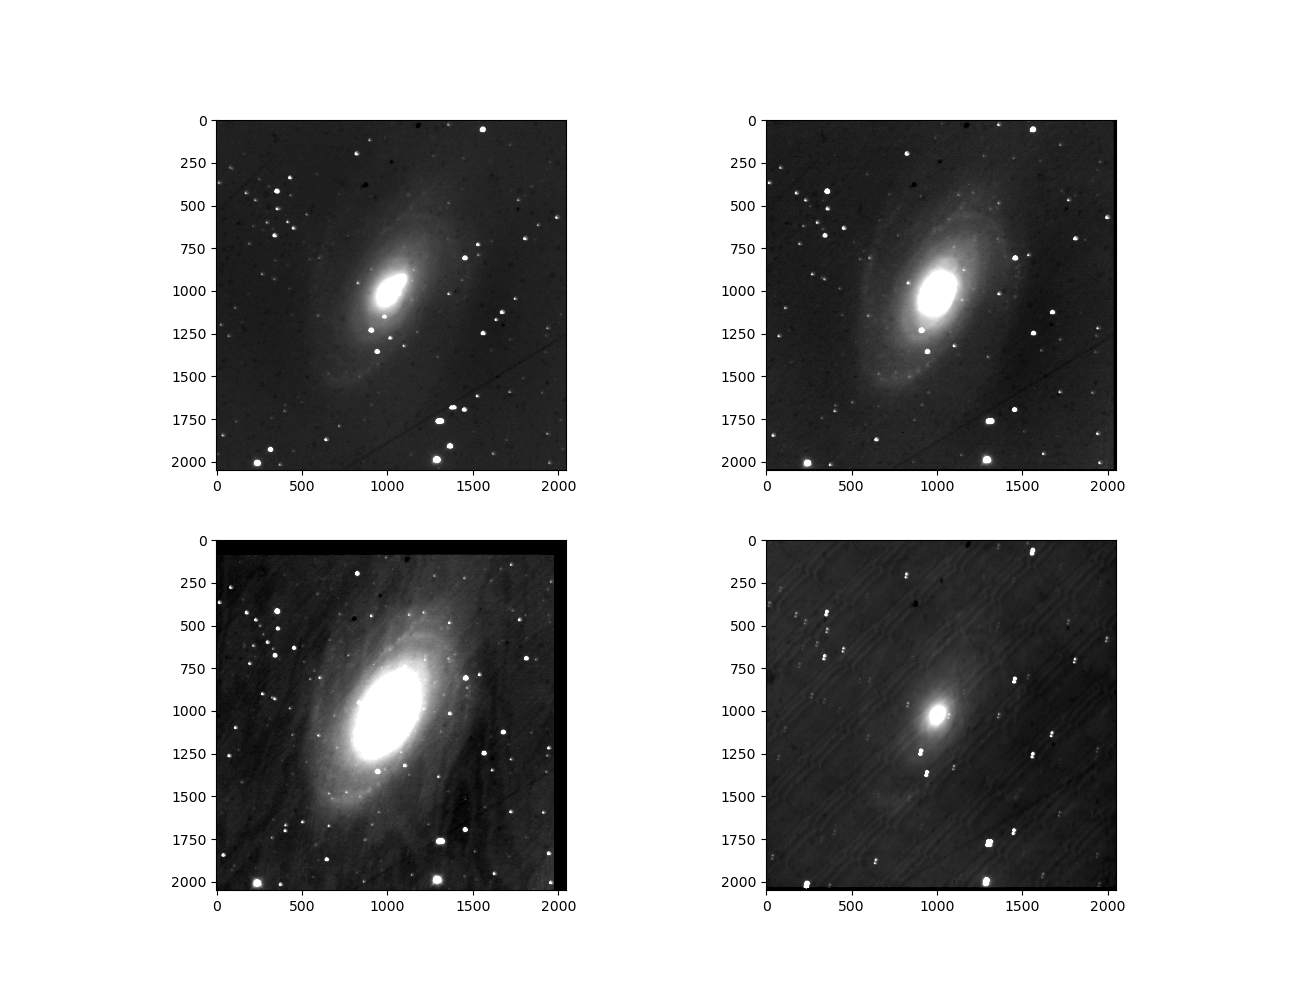
\includegraphics[scale=.4]{shifted_images.png}
    \caption{A plot of the reduced, shifted, and aligned images in each filter prior to stacking and compiling the final multi-color image. Looking at the bottom right plot, one can tell that it is the blue filter because of the minimal amount of light visible in the image, and the striations across the field of view. The bottom left plot seems to be the most saturated and seems to not be completely aligned with the rest of the images. The top two plots faintly display the spiral arms and seem to be more in focus than the bottom two.}
    \label{fig:shifted}
\end{figure}

\subsection{Complications}
% difficulties
When reducing the data, I learned the importance of having a consistent, standardized log that is organized and descriptive. Our files have inconsistencies in terms of file names and exposure times, which made the reduction process more difficult than it had to be, but I am grateful to have gone through this learning experience and will now know what to look out for moving forward. Another difficulty we encountered was due to the inexplicable striations produced by the blue filter, which caused abnormalities in the resulting stacked blue filtered image. The compiled multi-color image also seems to be slightly over-saturated, which is probably a result of a filter's exposure being too long.

\section{Analysis and Discussion}
When comparing the shifted images, I notice that the red filter collects the most amount of photons, as the image looks the largest in the bottom left plot, while the blue one collects the least. This makes sense, as red light has longer wavelengths than blue, making it easier for photons to reach the sensor. Another interesting thing to note is the fact that, though visible, the spiral arms appear faint in the final image. There are also a number of background stars out of focus in the field of view apparent at different colors.

\begin{figure}[h]
   \centering
    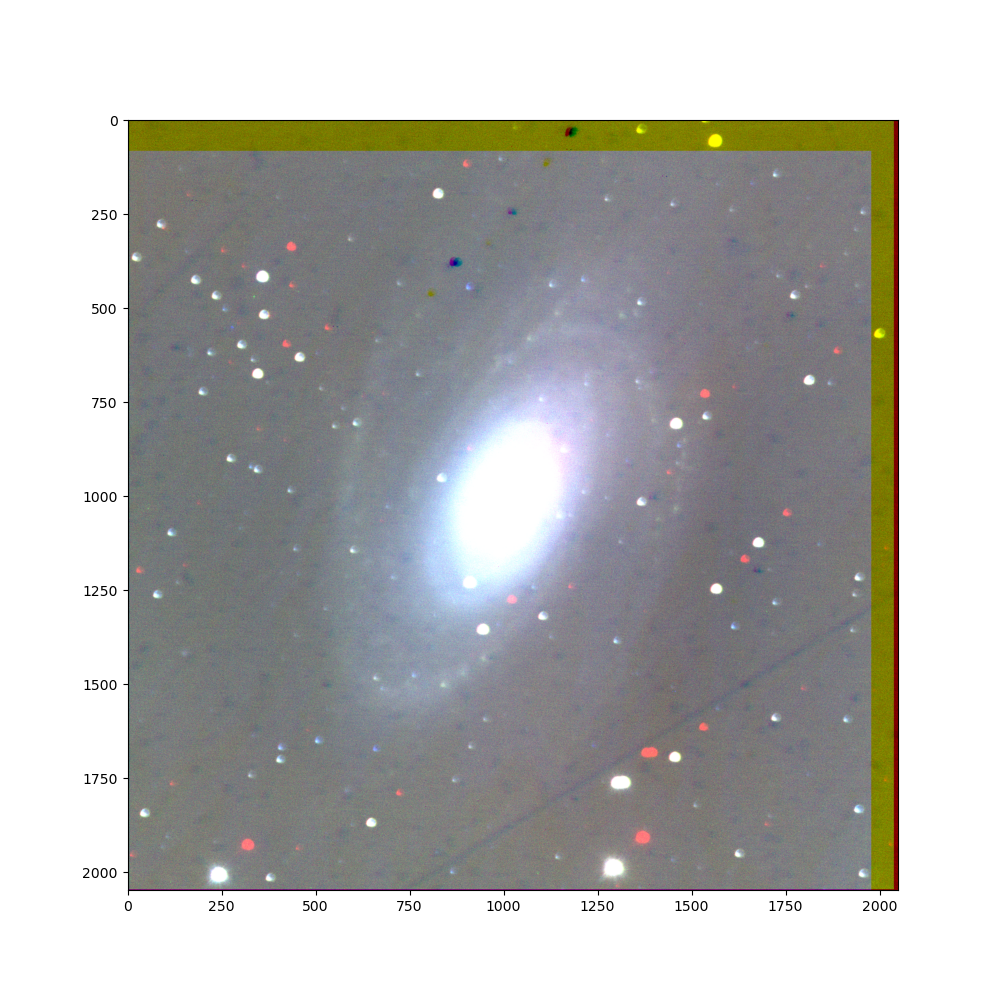
\includegraphics[scale=.4]{final_mci_image.png}
    \caption{The final multi-color image, compiled by stretching and stacking the four shifted images in each filter. The center of the galaxy is extremely bright and seems to be over-saturated, likely due to an exposure time being too long. One filtered image appears to be slightly off-centered in comparison to the other three images. I tinkered with the stretch and different colors to display until I was satisfied with the resulting image.}
    \label{fig:final}
\end{figure}

\subsection{Calculation}

According to Prof Chromey's textbook \textit{To Measure the Sky} \citep{Chromey_2016}, the relationship between the apparent magnitude $m$ and absolute magnitude $M$ of the same object is

\begin{align}
m - M &= 5 + \text{-}5 \log_{10}d
\end{align}

where $m - M$ is known as the distance modulus. This magnitude system quantifies brightness measurements on a logarithmic scale and gives the actual distance to the source in parsecs. Knowing that M 81 has an absolute magnitude of +6.94 \citep{nasa} and is located at a distance of 3.6 Mpc \citep{Gurzadyan}, we can easily calculate the absolute magnitude of the galaxy, defined as being the apparent magnitude that the source would have if it were at the standard distance of 10 pc in empty space \citep{Chromey_2016}.

\begin{align}
6.94 - M &= 5 + \text{-}5 \log_{10}(3.6* 10^6)\\
-M &= 5 + \text{-}5 \log_{10}(3.6* 10^6) - 6.94\\
M &= \text{-}5 + 5 \log_{10}(3.6* 10^6) + 6.94\\
M &= +34.7
\end{align}

\subsection{Conclusion}

I would have been interested in using the H$\alpha$ filter, which isolates and identifies ionized hydrogen within clouds of gas. According to a 2007 report on molecular clouds in the center of M 81, the galaxy contains HI and HII regions, and emmits CO; the molecular gas was first detected by Sage and Westpfahl in 1991 \citep{Casasola} and may have appeared in our images if we had used the H$\alpha$ filter. I would have also loved to dive a bit deeper into the spiral arms of the galaxy, possibly observing at different wavelengths to make them more visible. While the central bulge of M 81 contains older, redder stars, the arms are made of young, hot, bluish stars that formed within the last few million years \citep{nasa}. Comparing images taken of M 81 by the Hubble Space Telescope, the spiral arms are seen to wind all the way down to the central bulge. The supermassive black hole at the center of the galaxy is of great interet to me, as I am currently working on a South Pole Telescope project in collaboration with the Event Horizon Telescope focusing on the multiwavelength polarimetry of Sgr A* on short timescales. In comparison to the Milky Way, M 81* is roughly 15 times the mass of Sgr A* \citep{nasa} and because of the many similarities between the two \citep{Brunthaler}, findings of M 81* stated in the report may be applicable to Sgr A* as well. Overall, the completion of this project enhanced my observing methods and techniques, and the complications I faced taught me valuable lessons that will be applicable to future observational endeavors.



\bibliographystyle{acm}

\bibliography{citations}
\end{document}

